\documentclass[tikz,border=5pt]{standalone}
\usepackage{tikz, amsmath}
\usetikzlibrary{arrows.meta, calc}
\usepackage{stmaryrd}
\begin{document}
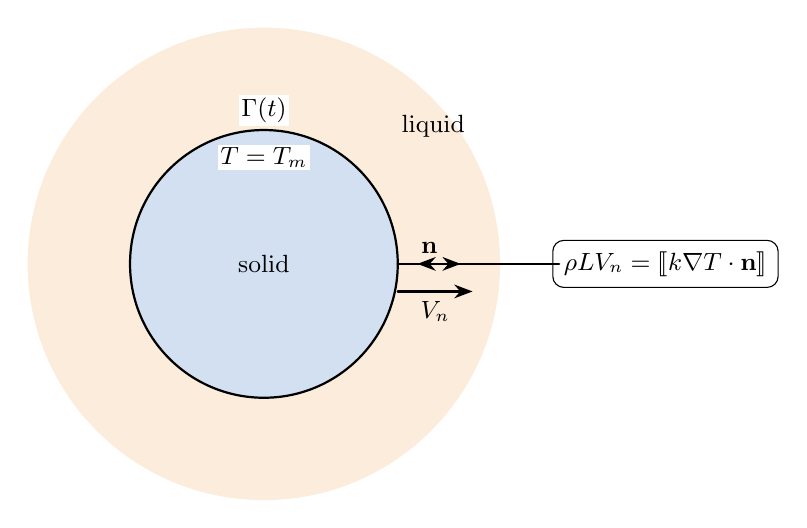
\begin{tikzpicture}[>=Stealth, line cap=round, line join=round, font=\small]
  \definecolor{solidcol}{RGB}{95,145,210}
  \definecolor{liquidcol}{RGB}{240,180,110}

  \def\R{1.7}
  \def\Rfar{3.0}

  \fill[liquidcol!25] (0,0) circle (\Rfar);
  \fill[solidcol!28] (0,0) circle (\R);
  \draw[thick] (0,0) circle (\R);

  \node at (0,0) {solid};
  \node at (2.15,1.75) {liquid};
  \node[fill=white, inner sep=1pt] at (0,1.95) {$\Gamma(t)$};
  \node[fill=white, inner sep=1pt] at (0,1.35) {$T=T_m$};

  \draw[->, thick] (\R,0) -- ++(0.8,0) node[midway, above] {$\mathbf n$};
  \draw[->, thick] (\R,-0.35) -- ++(0.95,0) node[midway, below] {$V_n$};

  \node[draw, rounded corners, fill=white, inner sep=4pt, align=center] at (5.1,0) {$\rho L V_n = \llbracket k\nabla T\cdot\mathbf n \rrbracket$};
  \draw[->, thick] (3.75,0) -- (1.95,0);
\end{tikzpicture}
\end{document}
